\chapter{\textit{Filter Bank Multicarrier} - FBMC} \label{capitulo3}

Este capítulo descreve a forma de onda FBMC. Este sistema é um tipo de tecnlogia FDM (\textit{frequency division multiplexing} - multiplexação por divisão na frequência), em que uma informação de banda larga é dividida em bandas mais estreitas, que ocupam alguns canais na frequência para serem transmitidas \cite{FDM}. Este tipo de multiplexação não é nenhuma novidade, mas, assim como os algortimos de FFT e IFFT popularizaram o OFDM, existem alguns recursos de processamento digital de sinais (DSP) que tornam o FDM e por conseguinte o FBMC mais atrativos no presente. A próxima seção mostra como isso acontece. 

\section{Processamento de Sinais Associado ao FDM}

\par Sinais de multiplexação em frequência tipicamente são criados através de estruturas como a da Figura \ref{trans_FDM}: 

\begin{figure}[h!]
\centering
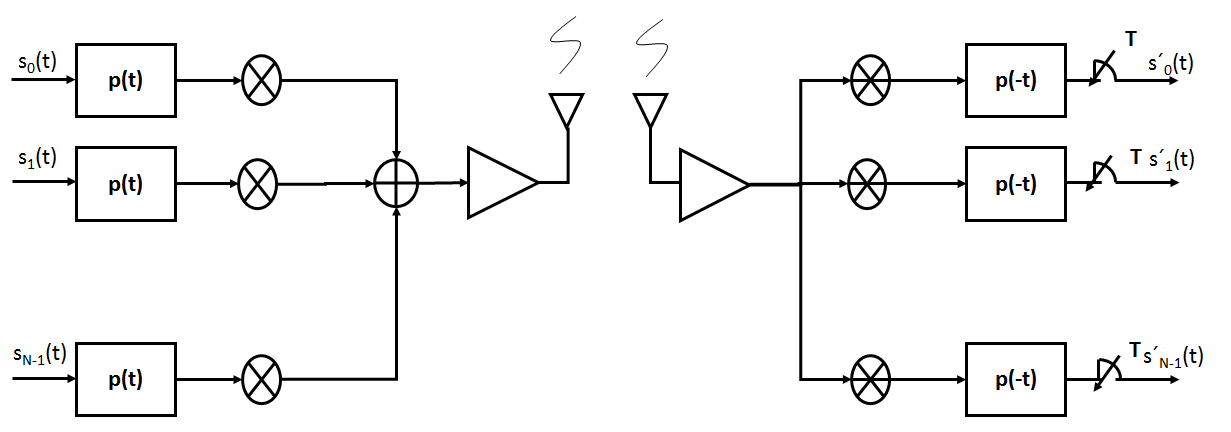
\includegraphics[width=3.5in]{transceptor_FDM.png} %Trocar para sistema FDM
\caption{Esquema de Transmissão e Recepção FDM}
\label{trans_FDM}
\end{figure}

\par Este tipo de sistema é bastante problemático. Observa-se que para que as sub-bandas mencionadas na introdução deste capítulo sejam transferidas aos seus canais correspondentes, cada ramo é multiplicado por uma frequência. O tipo de \textit{hardware} utilizado para realizar esta operação é o oscilador, um dispositivo altamente sensível a ruídos externos \cite{Boroujeny}. A consequência disto é que qualquer variação do ambiente externo resulta em desvios de frequência, o que dificulta a detecção correta do sinal, reduzindo a qualidade da informação obtida. Ilustrando melhor a dificuldade, para que a recepção fosse perfeita, cada ramo do receptor deveria ter um oscilador idêntico ao de transmissão, o que além de ser bastante complexo, envolve alto custo de implementação e gasto excessivo de energia, além de demandar bastante espaço nas estações móvel e base \cite{Krishna}.  O processamento digital do sinal FDM, tanto no processo de transmissão quanto no de detecção é uma alternativa interessante ao que foi descrito. A seguir, mostra-se como é possível utilizar esta ferramenta. 

\par Suponha que se deseja sub-amostrar um sinal discreto $x[n]$, amostrado do sinal contínuo $x_{c}[n]$, por um fator M. No domínio do tempo, esta operação é bastante simples, como mostra a Figura \ref{downsmp} e a equação \ref{downsmpeq} :

\begin{figure}[h!]
\centering
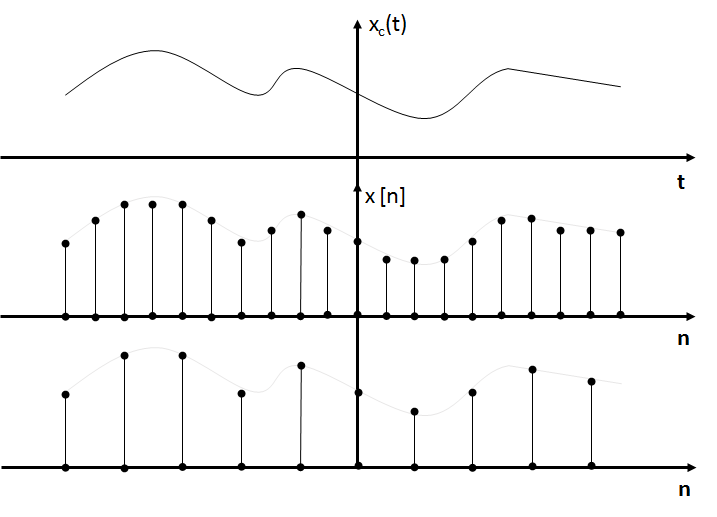
\includegraphics[width=3.5in]{DownSample.png} %Trocar para onda subamostrada
\caption{Exemplo de Subamostragem}
\label{downsmp}
\end{figure}

\begin{equation}\label{downsmpeq}
x_{d}[n] = x[Mn] 
\end{equation}

Suponha, ainda, que após a subamostragem, deseja-se aplicar ao sinal contínuo um filtro discreto $h[n]$, obtendo-se o sinal :

\begin{equation}
y[n] = \sum_{k=-\infty}^{\infty}x_{d}[k]h[n-k]
\end{equation}

É possível reescrever $y[n]$ como 

\begin{equation} \label{filt_sub}
y[n] = \sum_{k=-\infty}^{\infty}x_[k]h[nM-k]
\end{equation}

Guarde a equação \ref{filt_sub} e considere o seguinte: 

Uma sequência qualquer $u[k]$ pode ser reescrita fazendo-se k = rM + m, como $\sum_{m=0}^{M-1}$ $u[rM + m]$. A figura \ref{seq_poly} ilustra o processo:  

\begin{figure}[h!]
\centering
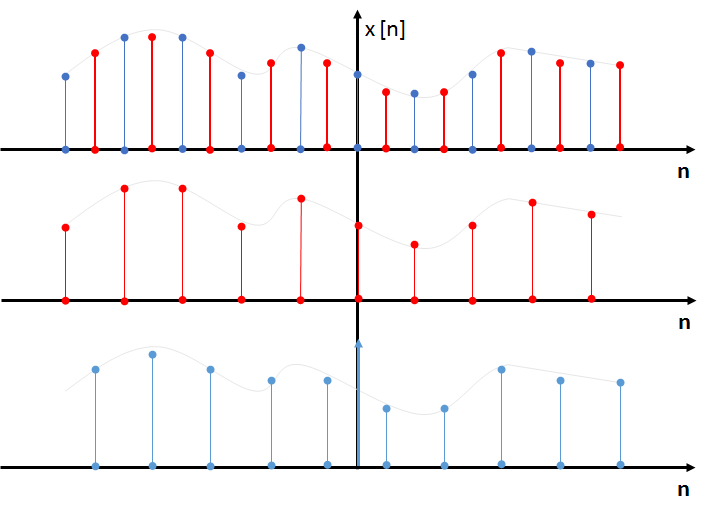
\includegraphics[width=3.5in]{seq_sub.png} % Construindo uma seq através de outra
\caption{Construção de uma sequência através de sub-sequências}
\label{seq_poly}
\end{figure}

Voltando a equação \ref{filt_sub} e aplicando-se o conceito da Figura \ref{seq_poly}, tem-se o resultado

\begin{equation} \label{conv_poly}
\begin{split}
y[n] &= \sum_{m=0}^{M-1}\sum_{r=-\infty}^{\infty}x_[rM+m]h[nM-rM+m] \\ 
     &= \sum_{m=0}^{M-1}\sum_{r=-\infty}^{\infty}x_[rM+m]h[(n-r)M+m] 
\end{split}
\end{equation}

Seja $x_m[r] = x[rM + m ]$ e $h_m[r] = h[rM + m]$, a equação \ref{conv_poly} pode ser reescrita como \cite{Kirshna}

\begin{equation} \label{conv_poly2}
\begin{split}
y[n] &= \sum_{m=0}^{M-1}\sum_{r=-\infty}^{\infty}x_{m}[r]h[n-r] \\ 
     &= \sum_{m=0}^{M-1}u_{m}[r]\ast h_{m}[r]
\end{split}
\end{equation}

Observa-se, então que é possível, quando da sub-amostragem (e também da super), filtrar-se partes de um sinal através de "sub-filtros". Tanto as "partes" ($u_{m}[n]$) quanto os "sub-filtros" ($h_{m}[n]$) são chamados componentes polifásicas. Este desenvolvimento será mantido em \textit{hold} por alguns instantes, enquanto se explora um outro tópico: o que acontece no domínio da frequência quando se sub-amostra um sinal? O porquê desta pergunta fará sentido em breve. 

Na Figura \ref{x_freq}, apresenta-se o espectro do sinal $x_{c}(t)$: 

\begin{figure}[h!]
\centering
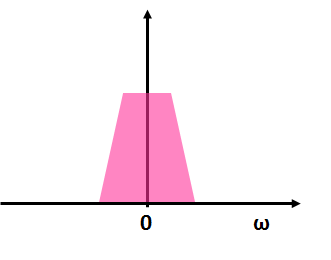
\includegraphics[width=2.5in]{spec_x.png} % espectro x_c(t)
\caption{Espectro de $x_c(t)$}
\label{x_freq}
\end{figure}
Amostrar este sinal no domínio do tempo, leva a expressão \cite{Krishna}
\begin{equation}
X(e^j\omega) = \frac{1}{T}\sum_{k=-\infty}^{\infty}\bigg[j\bigg(\frac{\omega}{T}-\frac{2\pi k}{T}\bigg)\bigg]
\end{equation}
no domínio da frequência, que é a transformada de Fourier de $x[n]$. 

A transformada de $x_{d}[n]$ apresenta resultado semelhante \cite{Krishna}: 
\begin{equation}
X_{d}(e^j\omega) = \frac{1}{T'}\sum_{k=-\infty}^{\infty}\bigg[j\bigg(\frac{\omega}{T'}-\frac{2\pi k}{T'}\bigg)\bigg]
\end{equation}
Fazendo-se $T'=MT$:
\begin{equation}\label{spec_sub}
X_{d}(e^j\omega) = \frac{1}{MT}\sum_{k=-\infty}^{\infty}\bigg[j\bigg(\frac{\omega}{MT}-\frac{2\pi k}{MT}\bigg)\bigg]
\end{equation}
Seria interessante escrever $X_{d}(e^j\omega)$ em termos de $X(e^j\omega)$. Isto e possível ao aplicar-se o conceito da Figura \ref{seq_poly} à equação \ref{spec_sub} - trocando-se a variável $k por rM + m$:

\begin{equation}\label{spec_sub1}
\begin{split}
X_{d}(e^j\omega) &= \frac{1}{M}\sum_{m=0}^{M-1}\frac{1}{T}\sum_{k=-\infty}^{\infty}\bigg[j\bigg(\frac{\omega - 2\pi m}{MT}-\frac{2\pi r}{T}\bigg)\bigg] \\
                 &= \frac{1}{M}\sum_{m=0}^{M-1}X(e^\frac{\omega - 2\pi m}{M})
\end{split}
\end{equation}

Graficamente, para M =2: 

\begin{figure}[h!]
\centering
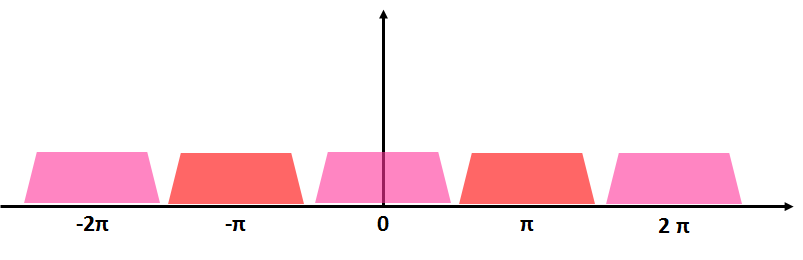
\includegraphics[width=2.5in]{sub_2.png} % espectro 2_fold
\caption{Espectro de $x_c(t)$ sub-amostrado}
\label{x_freq1}
\end{figure}

Observa-se que há alguns efeitos: alargamento da e repetição periódica da banda, além da redução da amplitude por um fator M. 
A resposta a pergunta anterior obtida, faz-se mais uma: qual a consequência, na frequência, de um atraso no domínio do tempo? Bom, esta correspondência é bastante conhecida. Considerando-se um sinal no tempo $u[n]$,  atrasa-lo no tempo por uma quantidade $p$ de amostras resulta em \cite{Krishna}:

\begin{equation}\label{delay}
x[n-n{0}] <-> X(e^j(\omega)e^{-j\omega n_p}
\end{equation}

Graficamente, para M = 2. 

\begin{figure}[h!]
\centering
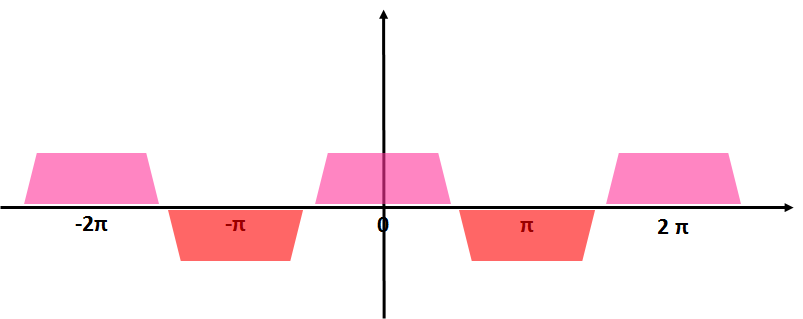
\includegraphics[width=3.5in]{sub_2_d.png} % espectro 2_fold + atraso
\caption{Espectro de $x_c(t)$ sub-amostrado com atraso}
\label{x_freq_atraso}
\end{figure}

Apresentou-se até agora diversos conceitos de processamento de sinais e chegou a hora de conectá-los. Na Figura \ref{polifase} desenha-se a equação \ref{conv_poly2}

\begin{figure}[h!]
\centering
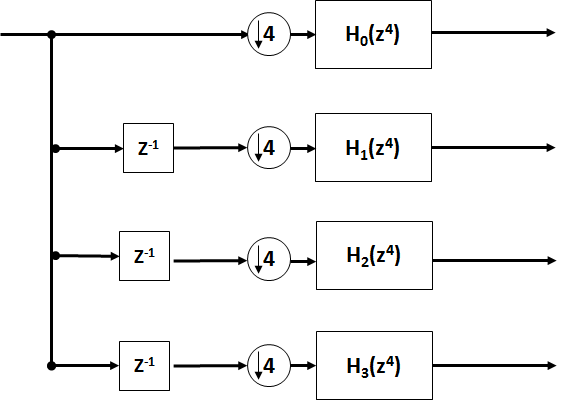
\includegraphics[width=3.5in]{filt_poli.png} % desenho filtro polifásico
\caption{Estrutura de Realização da Convolução por Componentes Polifásicas}
\label{polifase}
\end{figure}

Nesta figura, $H_{m}(zˆm)$ é a transformada-Z de $h_{m}[r]$.  

Viu-se que atrasos e sub-amostragem possuem alguns efeitos no espectro de um sinal ao qual essas operações são aplicadas. 
Na Figura \ref{efeitos}, explicitam-se estes efeitos para a primeira subportadora em cada ramo da Figura \ref{polifase}, admitindo como  entrada um sinal FDM como o de \ref{Espectro FDM}. Considere que as componentes $H_{m}(z^m)$ sejam filtros retangulares por simplicidade. 

\begin{figure}[h!]
\centering
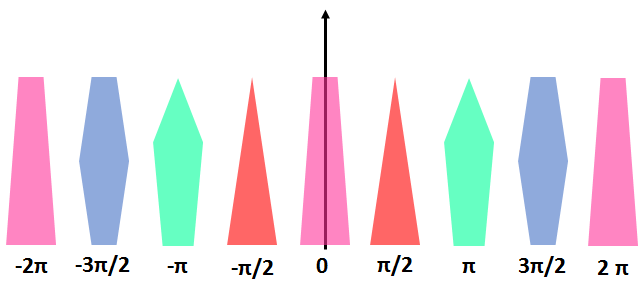
\includegraphics[width=2.5in]{spec_fdm.png} % espectro FDM
\caption{Espectro FDM}
\label{spec_fdm}
\end{figure}

\begin{figure}[h!]
\centering
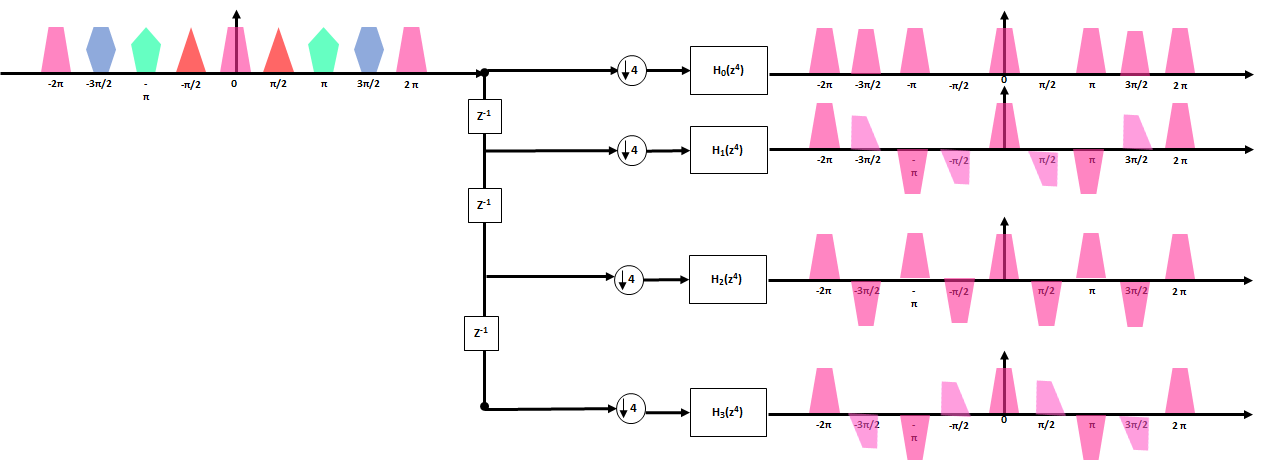
\includegraphics[width = 5.5in]{poli_filt_1.png} % desenho filtro polifásico
\caption{Estrutura de Realização da Convolução por Componentes Polifásicas}
\label{efeitos}
\end{figure}

\par Não é intuitivo perceber, mas se alimentarmos as entradas de um bloco de transformada de Fourier inversa (IDFT) com o resultado de cada ramo, será possível recuperar as sub-bandas do sinal FDM individualmente. A Figura \ref{rec_poli} exemplifica isso para o primeiro ramo. Mostra-se, então, que é possível, através de filtros polifásicos, criar-se um receptor FDM por meio do processamento digital de sinais. Este é apresentado na Figura \ref{estrutura_completa}. 

\begin{figure}[h!]
\centering
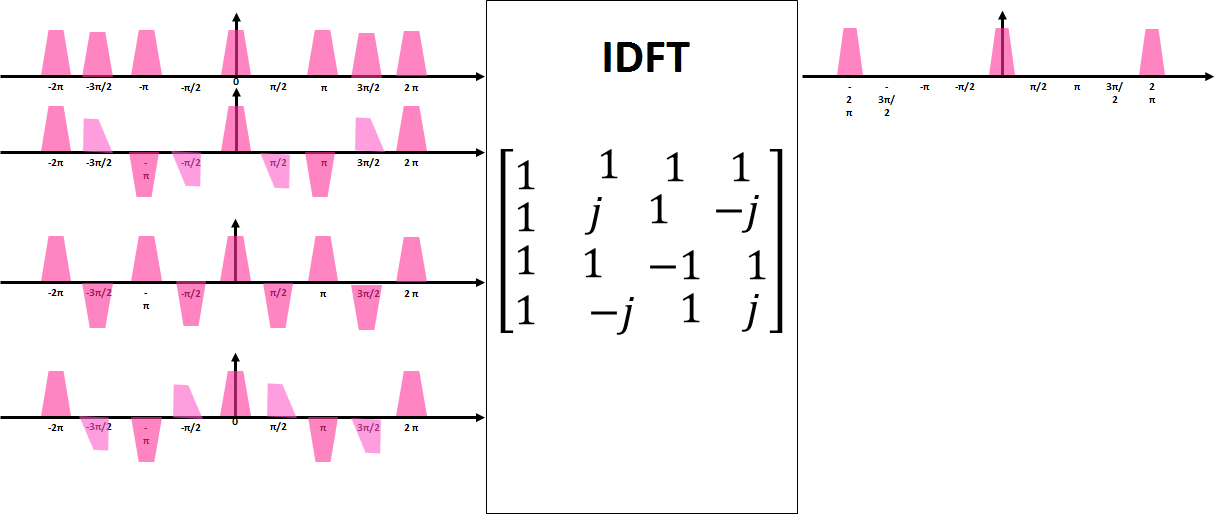
\includegraphics[width = 4.5in]{efeito.png} % desenho da soma
\caption{Receptor FDM com uso de Processamento de Sinais \cite{Krishna}}
\label{rec_poli}
\end{figure}

\par Como todas as operações aqui apresentadas são lineares, é possível desfaze-las através de operações inversas. Sendo assim, desde que os filtros H(z) atendam ao critério de Nyquist \ref{Saeed}, é possível criar um transmissor análogo ao receptor desenhado aqui. A próxima seção mostra um pulso que atende a esta condição e mostra que algumas adaptações necessárias a estrutura da figura \ref{estrutura_completa} por conta deste.  


\begin{figure}[h!]
\centering
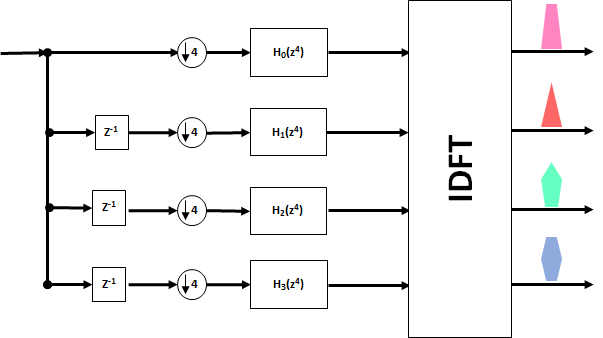
\includegraphics[width=3.5in]{estrutura_comp.png} % desenho soma 
\caption{Receptor FDM com uso de Processamento de Sinais \cite{Krishna}}
\label{estrutura_completa}
\end{figure}


\section{Formato de Pulso e Arquitetura de Transmissão/Recepção}

Finalizou-se a seção anterior apontando-se para o cuidado que se deve ter com o pulso $H(z)$. É bem sabido que o uso de filtros exije obediência aos critérios de Nyquist para que a seja possível detectar o sinal sem que haja erros. Estes critérios são dois \cite{Saeed}:

\begin{itemize}
\item critério ordinário 

\begin{equation}
h_{n}(t)\ast h_{n}^{\ast}(-t)\|_{t=kT} = \delta_{k} 
\end{equation}

\begin{equation}
\frac{1}{T}\sum_{m = -\infty}^{\infty}|H_{n}(j(\omega + m \frac{2 \pi}{T}))|^{2} = 1
\end{equation}

\item critério geral
\begin{equation}
h_{n}(t)\ast h_{n}^{*}(-t)|_{t=kT} = \delta_{k}\delta_{l-n} 
\end{equation}
\begin{equation}
\frac{1}{T}\sum_{m = -\infty}^{\infty}H_{n}(j(\omega + m \frac{2 \pi}{T}))H_{l}^{*}(j(\omega + m \frac{2 \pi}{T})) = \delta_{l-n}
\end{equation}

\end{itemize}
 
\par Desde a introdução desta dissertação, tem-se tentado mostrar a importância de pensar em formas de onda alternativas ao OFDM, para evitar o vazamento espectral, ter-se liberdade em relação ao sincronismo \ref{Bouroujeny} e entre outras razões. Uma ideia que naturalmente vem a cabeça é usar o OFDM com um filtro distinto da função retangular. Mostra-se a seguir porque isso não é uma alternativa: 

Seja

\begin{equation} \label{OFDM_pulso}
h_{n}(t) = q(t)e^{j\frac{2\pi nt}{T}} \cite{Saeed}
\end{equation}

um pulso aplicado ao diagrama da Figura \ref{OFDM_Trans}, em que q(t) não obedece a formatação retangular usual. Seja $Q(e^{j\omega}$) a transformada de Fourier de q(t), este pulso só atende aos critérios de Nyquist se respeitam as equações a seguir \cite{Saeed}: 

\begin{equation}
\frac{1}{T}\sum_{m = -\infty}^{\infty}|Q_{n}(j(\omega -n \frac{2 \pi}{T} + m \frac{2 \pi}{T}))|^{2} = 1
\end{equation}
\begin{equation}
\frac{1}{T}\sum_{m = -\infty}^{\infty}Q_{n}(j(\omega -n \frac{2 \pi}{T} + m \frac{2 \pi}{T}))Q_{l}^{*}(j(\omega -n \frac{2 \pi}{T} + m \frac{2 \pi}{T})) = \delta_{l-n} 
\end{equation}

\par Em \cite{Saeed} observa-se que estes critérios somente podem ser respeitados se $Q(e^{j\omega}) = 0$, que exije $|Q(e^{j\omega})| = 0$. Ou seja, a única forma de recuperar o sinal completamente é se o pulso $q(t)$ for nulo. Isto mostra que é inviável, com a estrutura crua do OFDM, utilizar um pulso alternativo. 
\par A conclusão anterior traz preocupações em relação ao desenho obtigo na Figura \ref{estrutura_completa}. Para que a recuperação do sinal seja perfeita, são necessárias algumas adaptações ao que se vê ali para o caso de $h(t)$ diferente da função $rect(t)$. Em \cite{Boroujeny2} e \cite{Bellanger}, apresentam-se o "cosine modulated multitone - CMT" e o "staggered modulated multitione - SMT", alternativas ao problema de atendimento aos critérios de Nyquist. As duas soluções mostram que:

\begin{enumerate}

\item Realizar uma multiplicação do tipo $\sum e^{(j \omega a\frac{\pi}{T})}$:

\begin{equation}
h_{n}(t) = q(t)\sum e^{(j \omega a\frac{\pi}{T}t)},
\end{equation}
em que $a$ é um inteiro qualquer, que resulta em:
\begin{equation}
H_{n}(e^{(j \omega}) = Q(j(\omega - \sum a\frac{\pi}{T} + n\frac{2\pi}{T})
\end{equation}

\item e além disso, utilizar-se da modulação O-QAM

\end{enumerate}
resultam no atendimento aos critérios geral e ordinário de Nyquist. 
\par Um modelo de filtro que ganhou popularidade na literatura FBMC relacionada ao 5G foi o projetado no PHYDAS \ref{Bellanger}. Este é apresentado a seguir:

\subsection{Formato de Pulso}

Como o filtro FBMC é o que o diferencia do OFDM, inicia-se a apresentação da forma de onda através do formato de pulso utilizado. Sabe-se que a IFFT/FFT possui um efeito de filtragem dos sinais a que é aplicada \cite{Boroujeny}. No domínio do tempo (discreto), pode-se representar este efeito da maneira a seguir \cite{Bellanger}:
\begin{equation}
y_{n} = \frac{1}{M}[x(n-M)+...+x(n-1)] = \frac{1}{M}\sum_{i=1}^{M}x(n-1),
\end{equation}
um filtro passa-baixa do tipo FIR (\textit{finite impulse response} - reposta ao impulso finita). No domínio da frequência \cite{Bellanger}:
\begin{equation}\label{eq_freq}
I(f) = \frac{sin\pi fM}{Msin\pi f}
\end{equation}

A equação \ref{eq_freq} é a fórmula matemática que leva ao espectro visto na figura \ref{fig_OFDM_freq}. A existências de lóbulos laterais de relativamente alta potência esbarra em algumas características que a forma de onda que transmitirá sinais 5G precisará ter. Recapitulando, isto é prejudical a sinais assíncronos, visto que representam um alto potencial para gerar interferências e assincronismo será fundamental no contexto da IoT \cite{Wunder}.  
\par Pensando nisso, procurou-se criar um tipo de filtro mais adequado. Baseou-se a escolha do pulso no critério de Nyquist, que no domínio da frequência significa simetria em relação a frequência de corte \cite{Bellanger}. 
\par Focando agora no processo de transmissão e recepção, para que este ocorra livre de erros, o filtro que transmite deve estar casado com aquele que recebe o sinal. Assim, utiliza-se "meio filtro" de Nyquist na saída e outro "meio filtro" na entrada. 
\par Com esses critérios em mente, desenhou-se alguns possíveis formatos para o pulso FBMC, chegando-se aos coeficientes abaixo: 

\begin{center} \label{coef_FBMC}
\begin{tabular}{ c c c c c c  }
 K & $H_{0}$ &  $H_{1}$ & $H_{2}$ & $H_{3}$ & $\sigma^{2}$ (dB) \\ 
 2 & 1 & $\frac{\sqrt{2}}{2}$ & - & - & -35\\  
 3 & 1 & 0.911438 & 0.411438 & - & -44\\
 4 & 1 & 0.971960 & $\frac{\sqrt{2}}{2}$ & 0.235147 & -65
\end{tabular}
\end{center}

Na tabela \ref{coef_FBMC}m, K representa o fator de superposição, ou seja, quantas amostras se sobrepõem em cada versão do filtro. Quanto maior for K, melhor localizado na frequência será o pulso. Para K = 4, tem-se a resposta da figura \ref{fig_FBMC}, no domínio da frequência:

5\begin{figure}[h!]
\centering
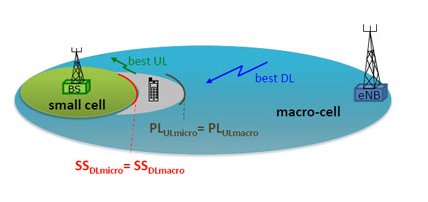
\includegraphics[width=3.5in]{comp.png} % Colocar o grafico das sub FBMC
\caption{Subportadoras FBMC}
\label{fig_FBMC}
\end{figure}

\par Nota-se uma expressiva redução da amplitude dos lóbulos laterais \cite{Bellanger}, um excelente benefício no contexto M2M. Em termos matemáticos, a forma de pulso se traduz em\cite{Bellanger}: 

\begin{equation}\label{eq_freq}
H(f) = \sum_{k=-(K-1)}^{K-1}H_{k}\frac{\sin(\pi(f-\frac{k}{MK}))}{MKsin(\pi(f-\frac{k}{MK}))}
\end{equation}

\par O próximo passo na construção da forma de onda FBMC é criar múltiplas subportadoras como a da \ref{fig_FBMC}, centralizadas em diferentes frequências. Isto é feito como mostra o diagrama de blocos da figura \ref{Trans_FBMC}. 

\begin{figure}[h!]
\centering
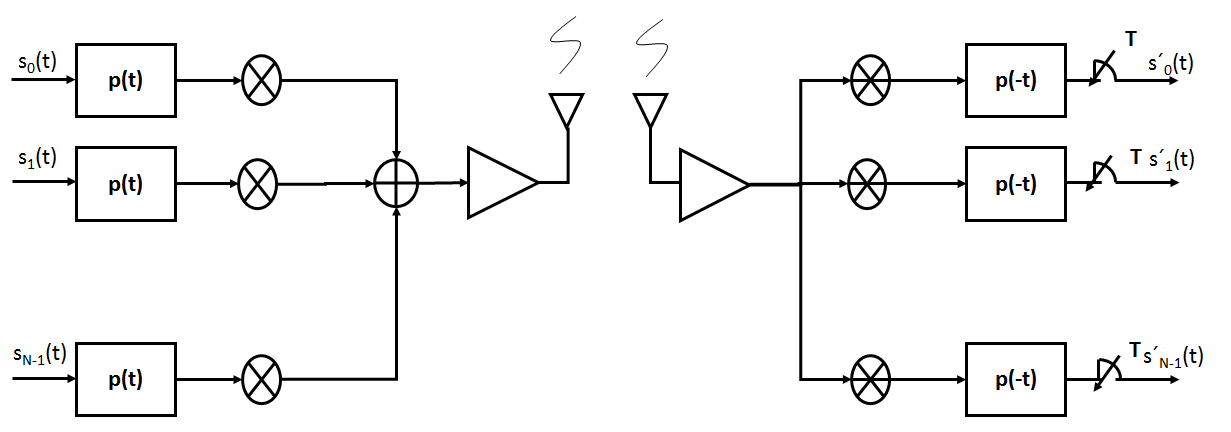
\includegraphics[width=3.5in]{transceptor_FDM.png}
\caption{Diagrama do Modem FBMC \cite{Boroujeny}}
\label{Trans_FBMC}
\end{figure}

\par Na seção do OFDM viu-se o quanto os algortimos de IFFT/FFT foram fundamentais no desenvolvimento da forma de onda tratada ali. Observando-se a Figura \ref{Trans_FBMC}, observa-se uma oportunidade de utilização da ferramenta, já que cada ramo é multiplicado por $\exp^{^{+}_{-} j2\pi}{f_{k}}$, $f_{k} = \frac{ft}{T}$ - coeficientes da transformada de Fourier. 


\subsection{Modulação O-QAM} 

Os símbolos FBMC criados através de \ref{simb_FBMC} geram interferência entre subportadoras adjacentes. Uma forma de evitar o problema é ocupar apenas subportadoras de subíndice par ou ímpar, mas nunca as duas simultaneamente \cite{Bellanger}. Isto representa um desperdício de espectro muito grande, fugindo completamente do propósito de se empregar uma nova forma de onda, já que um dos requisitos é a utilização desterecurso de forma mais eficiente. Uma alternativa possível é a modulação O-QAM (O - ortogonal), que faz com que duas subportadoras vizinhas sejam ortogonais, permitindo que se sobreponham sem que haja interferência no ponto de detecção do sinal. Este tipo de modulação é descrito a seguir.
\par Em sistemas usuais, tanto a parte imaginária quanto a parte real dos símbolos modulados digitalmente são transmitidas em conjunto. No O-QAM, é aplicado um atraso de meio período a uma das componentes do sinal de forma alternada - ora à parte real, ora à parte imaginária \cite{Bellanger}, conforme a figura \ref{O-QAM}. Isto faz com que canais adjacentes sejam sempre ortogonais uns aos outros, mas introduz algumas modificações a estrutura da Figura   \ref{simb_FBMC}.   
 
\begin{figure}[h!]
\centering
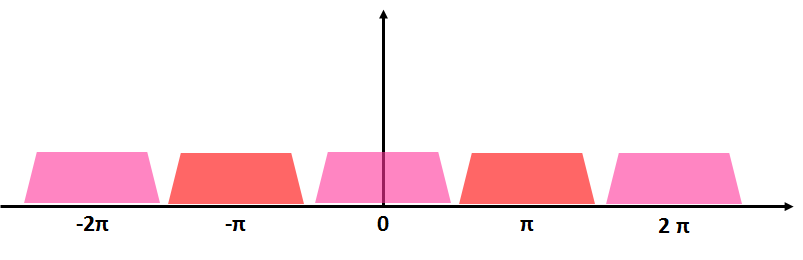
\includegraphics[width=3.5in]{sub_2.png} %trocar pela OQAM 
\caption{Modulação O-QAM}
\label{simb_FBMC}
\end{figure}

\par Observa-se que o sinal tem o dobro de amostras. Isto indica a primeira alteração: ao invés de super-amostrar o sinal por $M$ na estrutura da figura \ref{simb_FBMC}, que a propósito é o número de subportadoras, será necessário, apenas, a super-amostragem por $M/2$. Uma outra mudança é necessária, mas que não tem relação com o OQAM. 


\section{Desempenho sob o efeito de não linearidades }



















